\documentclass[11pt]{article}
\usepackage[margin=0.82in]{geometry}
\usepackage[utf8]{inputenc}
\usepackage[T1]{fontenc}
\usepackage{lmodern}
\usepackage{microtype}
\usepackage{amsmath,amssymb,amsfonts,mathtools}
\usepackage{booktabs,longtable,array,tabularx,multirow}
\usepackage{graphicx}
\usepackage{float}
\usepackage{enumitem}
\usepackage{xcolor}
\usepackage{hyperref}
\usepackage{caption}
\usepackage{fancyhdr}
\usepackage{titlesec}
\usepackage{lastpage}
\usepackage{siunitx}
\usepackage{url}
\hypersetup{colorlinks=true,linkcolor=blue,citecolor=blue,urlcolor=blue}
\pagestyle{fancy}
\setlength{\headheight}{14pt}
\fancyhf{}
\lhead{LogicFolding: No-Action Decision Memo}
\rhead{\thepage/\pageref{LastPage}}
\setlength{\parskip}{0.52em}
\setlength{\parindent}{0pt}
\setlist[itemize]{topsep=2pt,itemsep=2pt,leftmargin=*}
\setlist[enumerate]{topsep=2pt,itemsep=2pt,leftmargin=*}
\titleformat{\section}{\Large\bfseries}{\thesection}{0.6em}{}
\titleformat{\subsection}{\large\bfseries}{\thesubsection}{0.6em}{}
\titleformat{\subsubsection}{\normalsize\bfseries}{\thesubsubsection}{0.6em}{}
\newcommand{\R}{\mathbb{R}}
\newcommand{\dd}{\,\mathrm{d}}
\newcommand{\argmin}{\operatorname*{arg\,min}}
\newcommand{\norm}[1]{\left\lVert #1 \right\rVert}
\newcolumntype{Y}{>{\raggedright\arraybackslash}X}

\title{\textbf{LogicFolding as a No-Action Decision Memo}\\
\large A trading, investment, and engineering-allocation screen after third-pass red-team review}
\author{Regenerated technical write-up, version 4.1}
\date{May 27, 2026}

\begin{document}
\maketitle

\begin{abstract}
This fourth version replaces the earlier ``portable methodology,'' ``falsification roadmap,'' and ``decision-screen roadmap'' with a stricter conclusion: LogicFolding-style 3D-native logic folding fails the test of an actionable trading, investment, or engineering-allocation thesis today. The third-pass red-team review argues that Gate 0 names an unavailable business partnership rather than a technical test; that passing Gate 0 would not make the later physics, thermal, yield, APC, and EDA gates likely; that the thermal kernel and APC models were not operational; that the cost gate must be joint with sustained performance; and that independent reproduction is impossible without an open reference implementation. This memo accepts those objections. It converts the output into a default 
\textbf{NO ACTION} recommendation, with only three kinds of public evidence capable of reopening the case: (i) teardown and measurement of a shipping product showing sustained time-constant improvement and thermal viability, (ii) a publicly identified manufacturing partner for dual-active-logic stacking with disclosed or escrowed data rights, and (iii) an open-source reference flow runnable on public PDKs and benchmarks. The memo remains technically explicit, but it no longer pretends that elegant equations, operator notation, or proposed interfaces make the hypothesis practically testable.
\end{abstract}

\tableofcontents
\clearpage

\section{Executive decision}
\textbf{Decision output today: No trade. No allocation. No engineering adoption. Ignore for investment purposes until public evidence changes.}

The earlier documents were progressively downgraded from a proposed portable methodology to a falsification roadmap and then to a decision screen. The third-pass red-team review shows that even this decision-screen framing remained too optimistic. It identified a fatal practical issue: the precondition for testing the hypothesis is a business partnership involving a leading-edge foundry or integrated manufacturer, proprietary process data, active-logic stacking capability, and an open or escrowed EDA flow, well beyond what any technical plan can specify \cite{UserRedTeam3}. No ordinary investor, academic group, or fabless team can verify such a condition independently.

Therefore the correct form of the document is a \textbf{no-action decision memo} that specifies what public evidence would be needed to reopen the case, rather than a ``how to test LogicFolding'' technical plan. The value of the document is negative screening: it prevents a press release or speculative roadmap from being misread as evidence of a new portable scaling paradigm.

\begin{figure}[H]
\centering
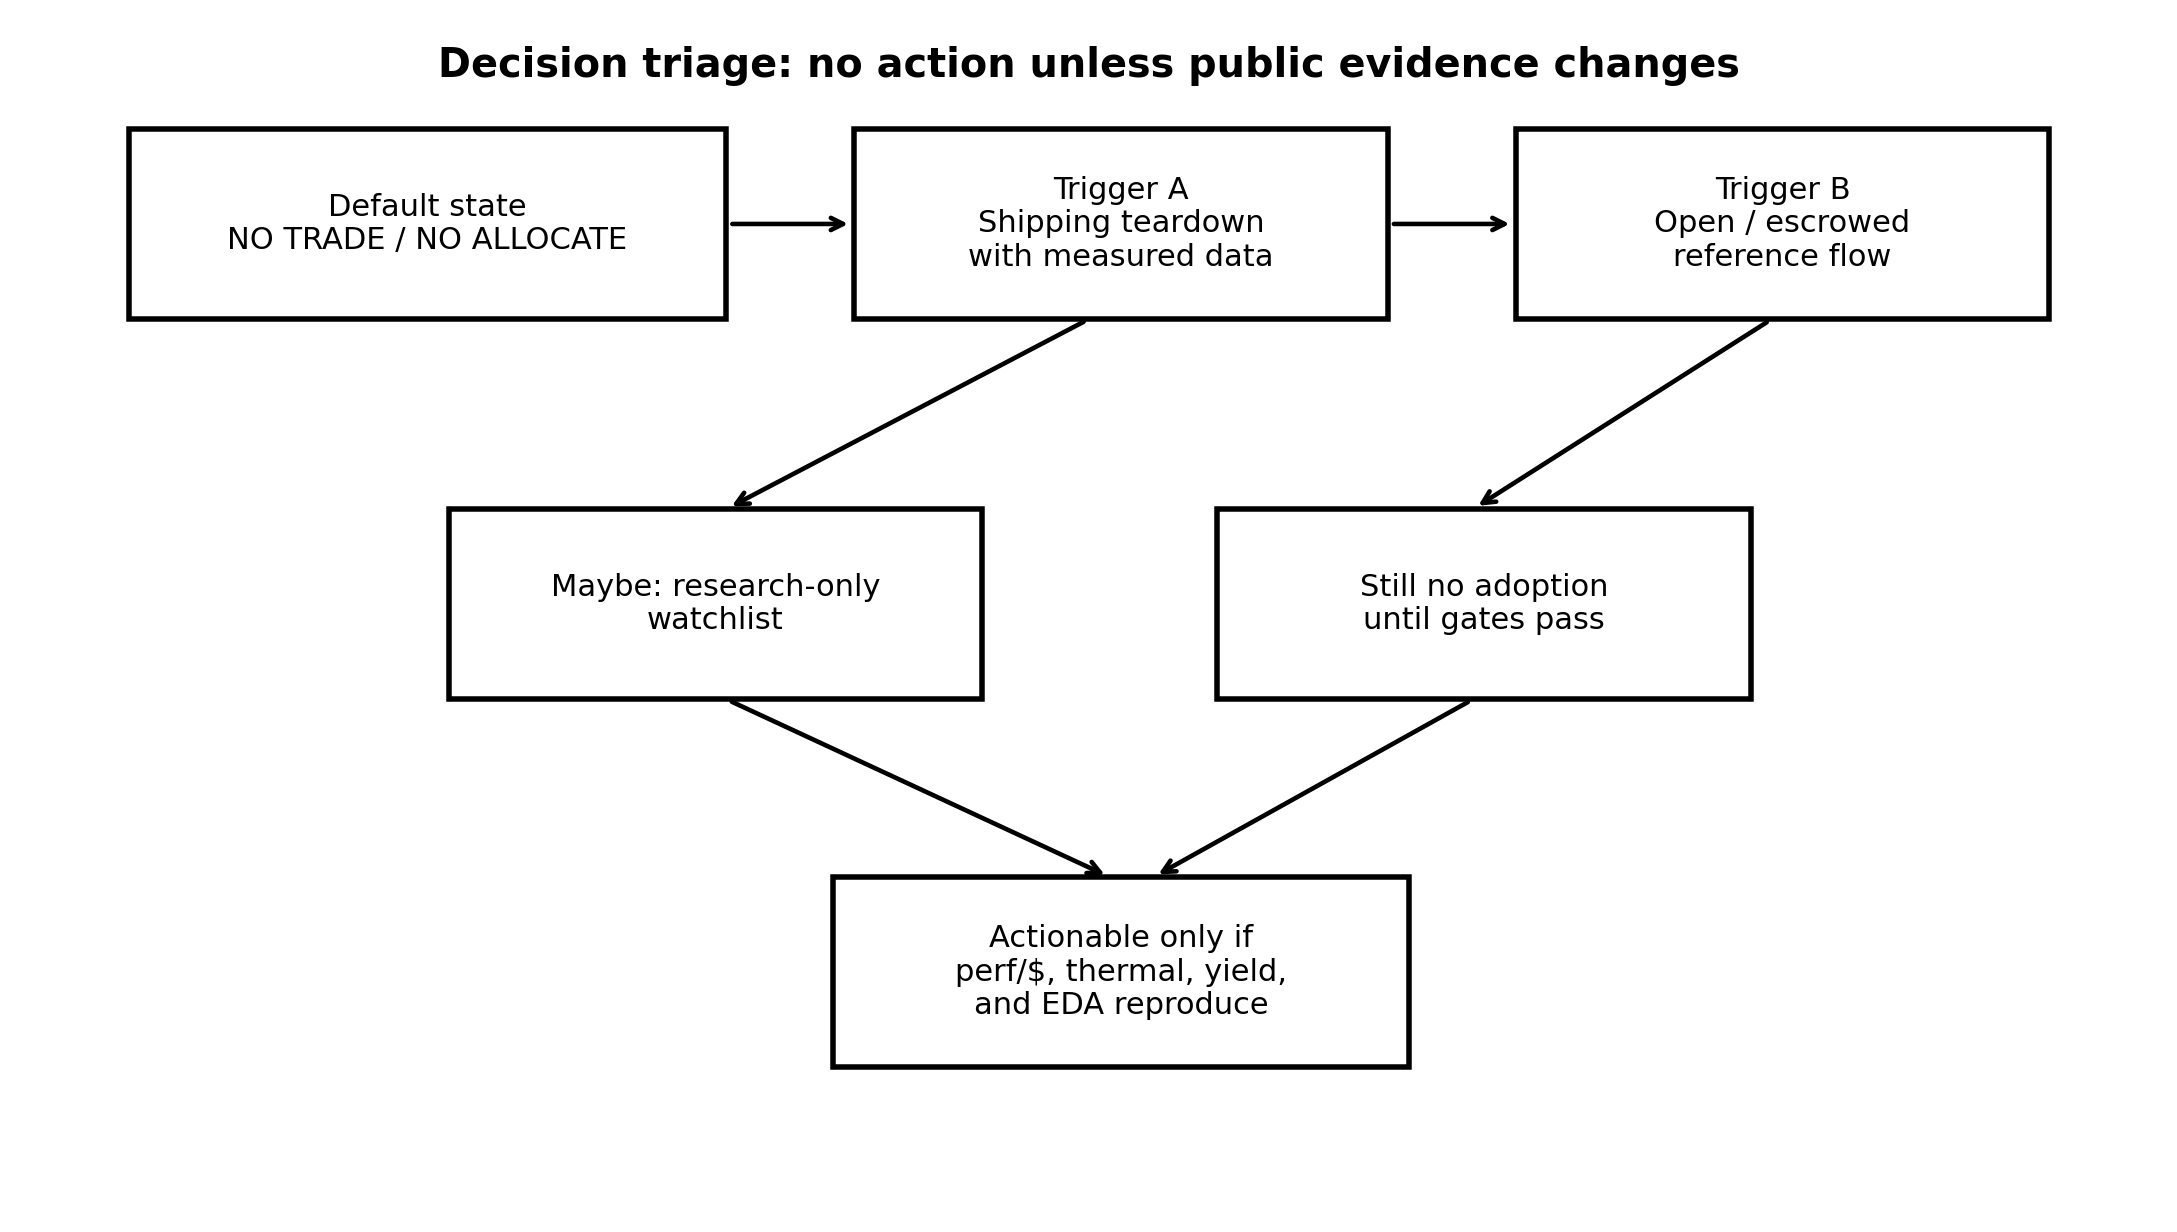
\includegraphics[width=0.98\linewidth]{fig_triage.png}
\caption{The current action is NO. The case can only be reopened by observable evidence, not by additional abstractions.}
\end{figure}

\subsection{One-sentence thesis}
LogicFolding is an interesting hypothesis about direct path-time reduction, actionable only after a shipping product or open reference implementation provides measured evidence that the gains exceed vertical parasitic, thermal, yield, cost, EDA, and control penalties.

\subsection{Immediate implication for readers}
\begin{itemize}
  \item \textbf{Trader:} do not trade on Tau Scaling or LogicFolding claims without product teardown evidence.
  \item \textbf{Investor:} do not allocate capital to the hypothesis unless diligence obtains foundry data rights and a credible manufacturing path.
  \item \textbf{Engineering manager:} do not divert a product team from backside power, chiplets, conventional 2.5D/3D packaging, or node/platform work.
  \item \textbf{Research team:} treat this as a narrow research question, not as a development program.
\end{itemize}

\section{Why the conclusion changed}
Huawei's public Tau Scaling statement frames LogicFolding as a circuit-level approach to reducing critical-path wiring and signal time constant, while Reuters reported that Huawei did not provide independent performance validation and that heat, power, cost, system integration, and tools remain obstacles \cite{Huawei2026,Reuters2026}. Prior versions of this report treated those claims as a motivation for a portable methodology, then as a falsification roadmap.

The first and second red-team reviews forced the central downgrade: the methodology was not production-ready, the gates were not sufficiently quantified, the EDA stack did not exist, and independent falsification required data that most researchers could not obtain \cite{UserRedTeam1,UserRedTeam2}. The third-pass review adds the final correction: a decision screen that can only say ``no'' or ``not testable'' is not a useful allocation tool unless it explicitly becomes a no-action memo with concrete triggers for reopening \cite{UserRedTeam3}.

\section{No-adoption statement}
\textbf{A foundry, EDA vendor, investor, or fabless team reading this today should not implement LogicFolding-style design as a production flow or fund it as a near-term alternative to backside power or conventional advanced packaging.}

This statement is a claim that the evidence package is missing, leaving open whether the physics is possible in some cases. A production allocation requires:
\begin{enumerate}
  \item independent silicon measurements;
  \item sustained workload thermal maps;
  \item measured vertical parasitics and path-time break-even;
  \item composite yield, test, and DPPM evidence;
  \item a credible manufacturing supply chain;
  \item an EDA flow that can be reproduced outside the inventing team;
  \item a joint performance-per-watt-per-cost advantage over a planar or platformized alternative.
\end{enumerate}

None of these are established by a press release, a paper architecture, or a mathematical framework.

\section{Gate 0 is an unavailable partnership}
Earlier versions called Gate 0 a precondition: identify a manufacturer and obtain data rights. The third-pass red-team review is correct that this language made Gate 0 sound like a normal technical milestone. Gate 0 is in fact a business partnership requiring unusual disclosure of proprietary process information \cite{UserRedTeam3}.

\subsection{What a real partnership would need}
A credible Gate 0 package would require, at minimum:
\begin{longtable}{p{0.22\linewidth}p{0.68\linewidth}}
\toprule
\textbf{Area} & \textbf{Required evidence or right}\\
\midrule
\endfirsthead
\toprule
\textbf{Area} & \textbf{Required evidence or right}\\
\midrule
\endhead
Manufacturing partner & Named foundry or integrated manufacturer willing to run dual-active-logic test vehicles.\\
Data rights & Contractual access to vertical via parasitics, bond quality, overlay fields, defect maps, yield tails, thermal test structures, and failure analysis.\\
IP framework & Clean-room or escrow arrangement specifying who owns partitioning algorithms, process improvements, metrology data, and failed design information.\\
EDA terms & Access to extraction, timing, thermal, DFT, and reliability hooks sufficient to build a reproducible flow.\\
Publication or audit & Third-party audit or public summary that reports enough data to support investment conclusions without revealing trade secrets.\\
\bottomrule
\end{longtable}

Without such a package, a reader cannot evaluate progress. The condition is binary and currently unverified. The rational output is ``ignore unless the partnership itself becomes public or auditable.''

\section{Expected value remains negative even if Gate 0 appears}
Passing the business-partnership precondition would not imply technical feasibility. It would merely make testing possible. The correct decision model is conditional:
\begin{equation}
P(\mathrm{success}) = P(G_0)P(G_P\mid G_0)P(G_T\mid G_0,G_P)P(G_Y\mid \cdots)P(G_E\mid \cdots)P(G_C\mid \cdots),
\end{equation}
where $G_0$ is the partnership/data gate, $G_P$ is the parasitic break-even gate, $G_T$ is the thermal gate, $G_Y$ is the yield/test gate, $G_E$ is the EDA/reproducibility gate, and $G_C$ is the cost/performance gate.

A press release can raise interest in one term, but an investment decision must multiply all terms. If any term is close to zero, the total remains close to zero.

\begin{figure}[H]
\centering
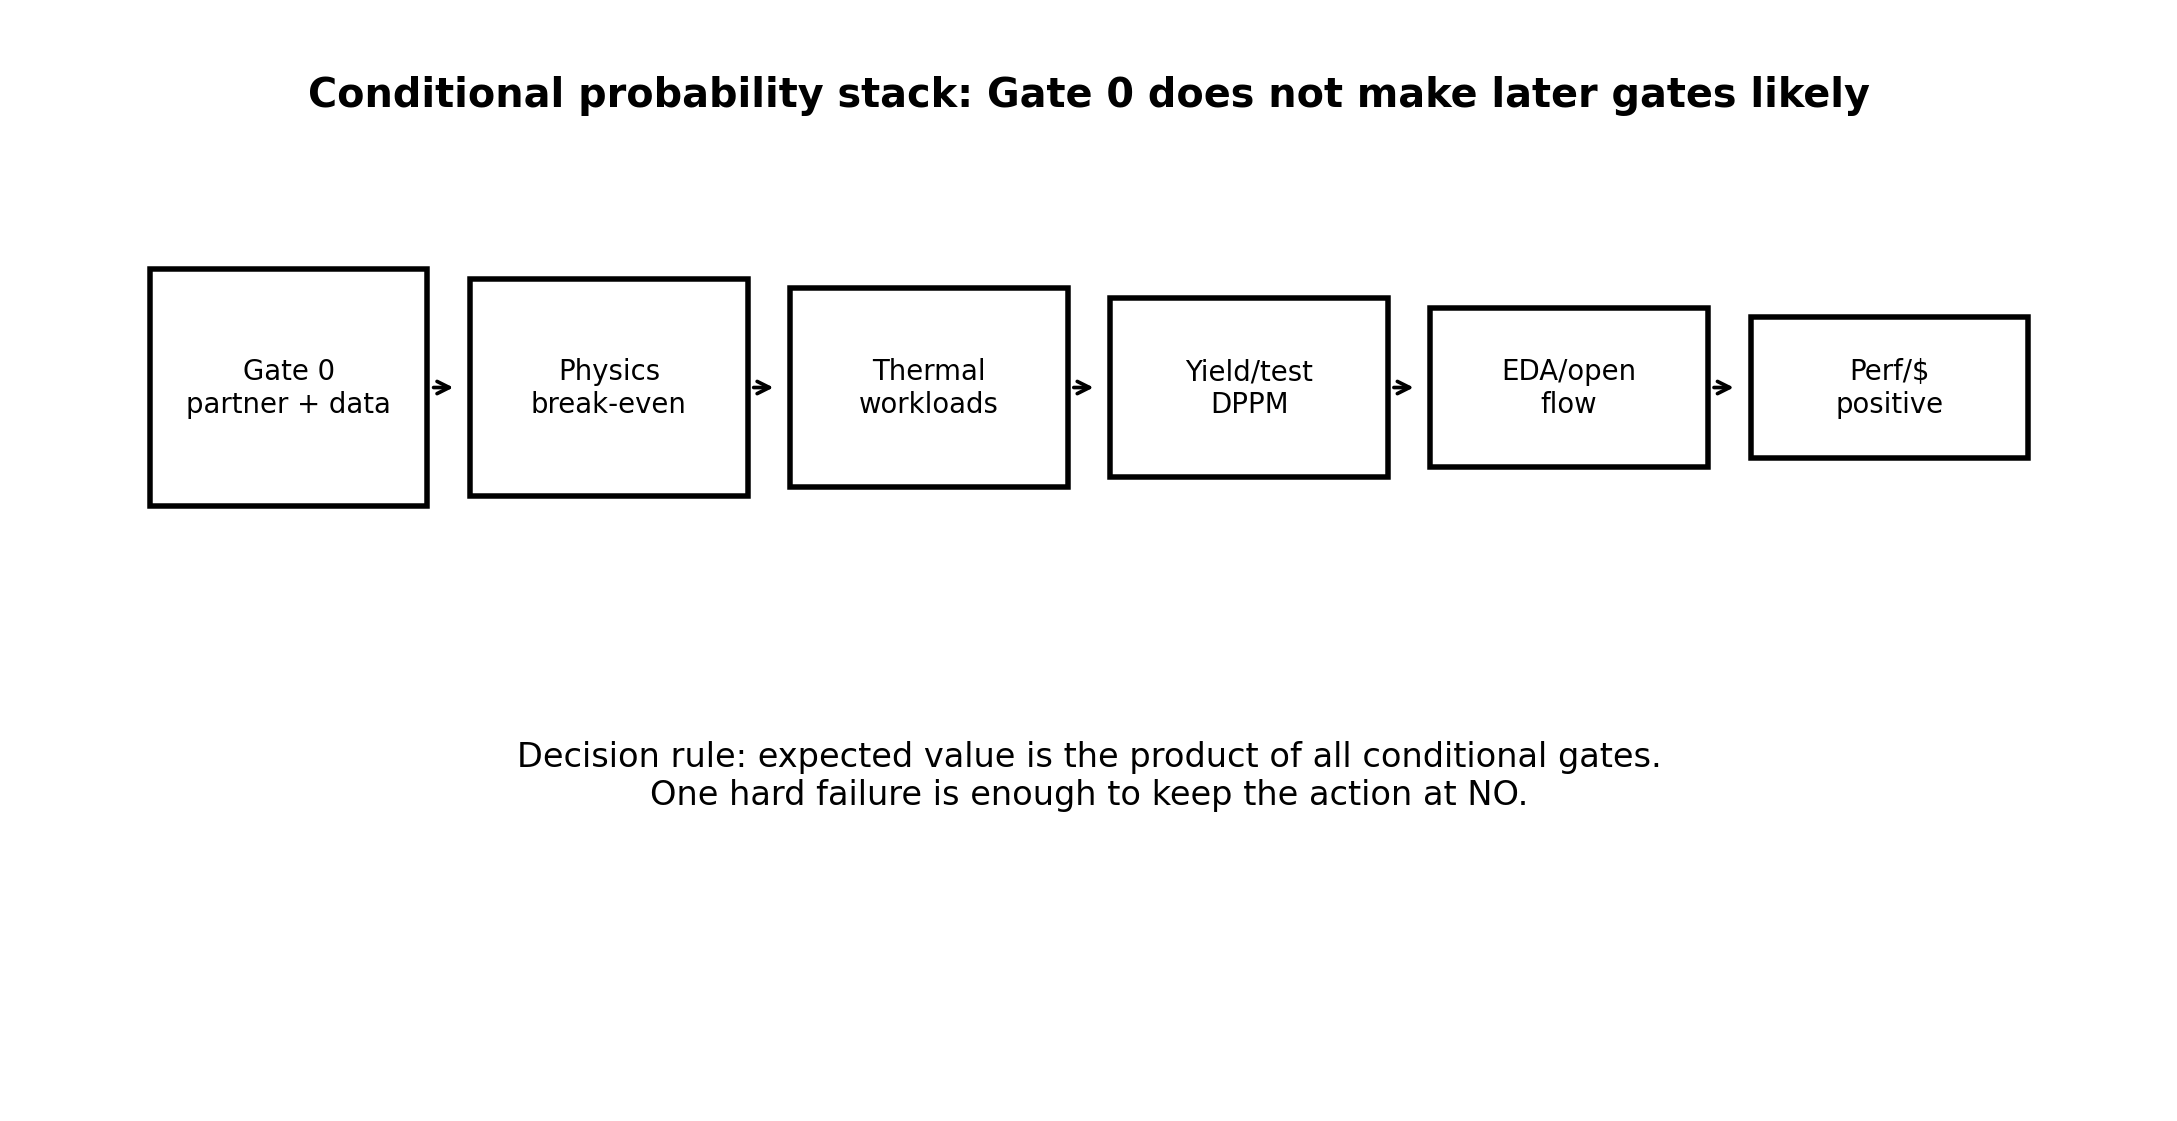
\includegraphics[width=0.98\linewidth]{fig_ev.png}
\caption{Gate 0 only permits testing. It does not make the physics, yield, EDA, or cost gates likely.}
\end{figure}

\section{Observable triggers that can reopen the case}
The conclusion is closed until observable triggers appear; reopening requires public evidence rather than further abstraction.

\begin{longtable}{p{0.18\linewidth}p{0.34\linewidth}p{0.36\linewidth}}
\caption{Reopen triggers and required evidence.}\\
\toprule
\textbf{Trigger} & \textbf{What must appear} & \textbf{Why it matters}\\
\midrule
\endfirsthead
\toprule
\textbf{Trigger} & \textbf{What must appear} & \textbf{Why it matters}\\
\midrule
\endhead
Shipping teardown & A real product teardown showing folded active logic, not just packaging, plus independent measurements of path delay, power, thermal behavior, and die/package cost. & Converts the hypothesis from press-release claim to measured product evidence.\\
Foundry disclosure & A named manufacturer offering or piloting dual-active-logic stacking with auditable data access. & Converts Gate 0 from impossible business precondition to a testable project.\\
Open reference flow & Open-source 3D-native partitioning and proxy signoff runnable on public PDKs and benchmarks. & Establishes methodological soundness, even if advanced-node feasibility remains unproven.\\
Sustained workload data & Ten-minute or longer workloads such as video encode, AI inference, gaming, and modem/camera stress with thermal maps. & Distinguishes burst benchmark wins from consumer-product viability.\\
Perf/\$ evidence & Sustained performance-per-watt divided by cost per good die beats the planar/platformized alternative. & Prevents costly low-value folding strategies from passing a cost-only screen.\\
\bottomrule
\end{longtable}

Until at least one of the first three triggers appears, the correct monitoring posture is low-effort watchlist only.

\section{Vertical break-even: do not use arbitrary targets}
Earlier versions used illustrative values for vertical $RC$ targets. The third-pass red-team review correctly objects that such targets are not credible without measured data and that fine-grained folding may usually lose once vertical overhead is included \cite{UserRedTeam3}.

A path-level break-even test must be written with measured or extracted quantities:
\begin{equation}
\Delta \tau_{save}(\ell_h) > N_v(R_v C_{load}+R_{drv}C_v+R_v C_v) + N_b(R_b C_{load}+R_{drv}C_b+R_b C_b) + \Delta \tau_{red} + \Delta \tau_T,
\label{eq:breakeven}
\end{equation}
where $\Delta \tau_{save}(\ell_h)$ is horizontal delay saved by shortening a wire of effective length $\ell_h$, $N_v$ is vertical via count, $N_b$ is bond/contact count, $\Delta \tau_{red}$ is redundancy overhead, and $\Delta \tau_T$ is thermal derating of delay.

The gate is path-level, not parameter-level. Specifically:
\begin{quote}
For the actual folded paths, under measured parasitics and temperature derates, Eq. \ref{eq:breakeven} must hold for enough critical paths to improve sustained system performance per watt after area, yield, and cost penalties.
\end{quote}

If only very long global paths pass, the approach may be a niche floorplanning technique rather than a standard-cell-level scaling law. If typical CPU or NPU timing paths fail, the architecture is not economically interesting.

\section{Thermal model: replace the lumped boundary with a calibrated workload test}
A single lumped area-normalized resistance cannot validate active-on-active logic. The thermal response must be local, spatial, temporal, and workload-specific. Define a workload $W$ with power-density field $p_W(r,t)$ and a temperature response
\begin{equation}
\Delta T_W(r,t)=\int_{0}^{t}\int_{\Omega} K(r,r',t-s)p_W(r',s)\,\dd r'\dd s,
\label{eq:kernel}
\end{equation}
where $K$ is a calibrated thermal kernel for the specific stack, package, and cooling envelope.

\begin{figure}[H]
\centering
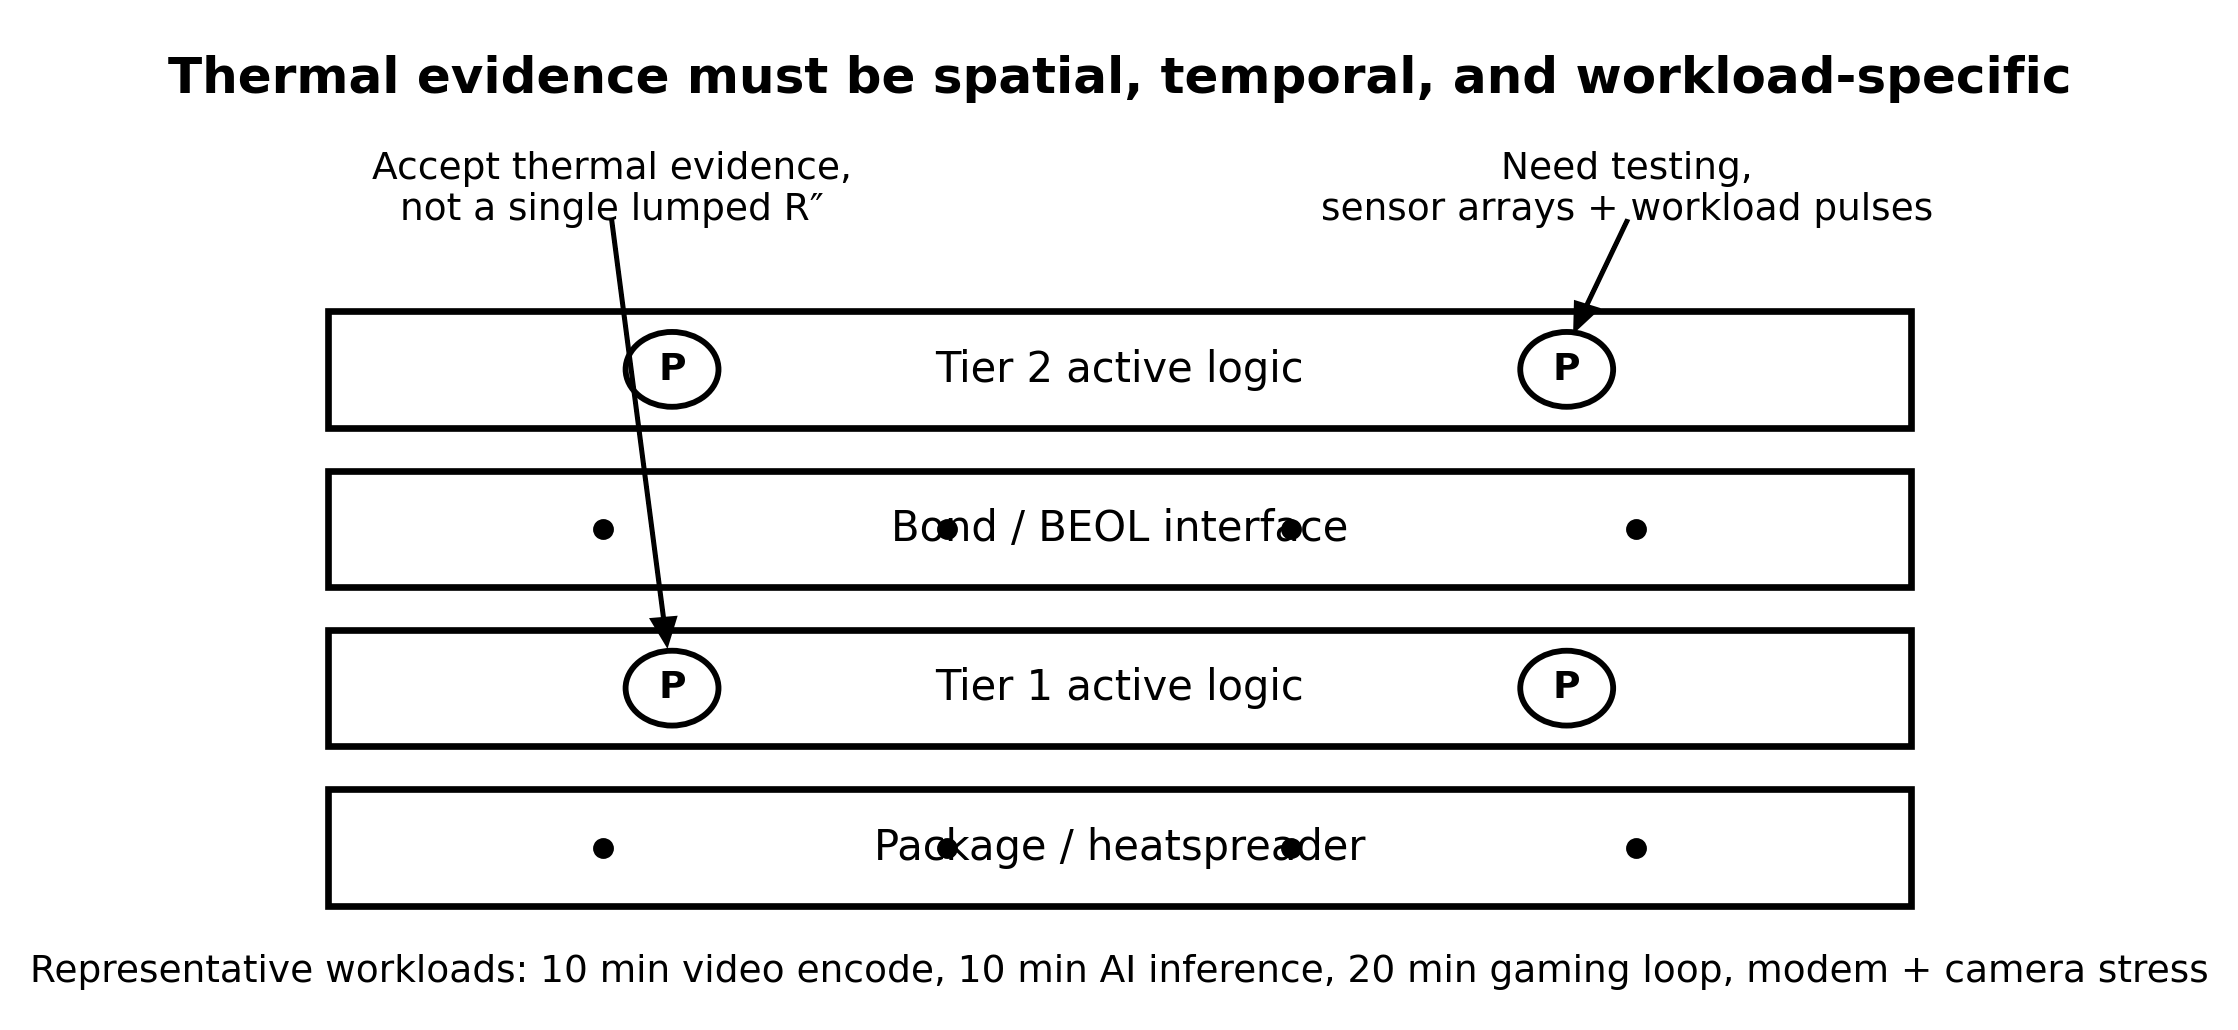
\includegraphics[width=0.98\linewidth]{fig_thermal_kernel.png}
\caption{Thermal validation requires spatial and temporal calibration. A lumped number can only be an early warning, not an acceptance gate.}
\end{figure}

\subsection{Calibration requirements}
A falsifiable thermal gate must specify:
\begin{itemize}
  \item a thermal test vehicle with heater/sensor arrays near folded active regions;
  \item sensor spacing and time resolution sufficient to resolve hotspot gradients and burst/sustained transitions;
  \item package and cooling boundary conditions, including heat spreader, TIM, chassis, and skin-temperature limits;
  \item workload set: at least 10 minutes of video encode, 10 minutes of sustained AI inference, 20 minutes of gaming loop, and a modem/camera stress case;
  \item an acceptance metric such as $\Pr[\max_{r,t\in W}T(r,t)>T_{limit}]<\epsilon$ and a maximum permitted throttling fraction.
\end{itemize}

Without these, the kernel is decorative. With them, thermal evidence becomes a real screen. The same chip can pass burst benchmarks and fail sustained workloads. Therefore burst scores are not investment evidence.

\section{APC is an unsolved research blocker}
The earlier APC section still implied that a reduced-order model could be engineered into a gate. The third-pass red-team review is right to reject that. Spatial APC for folded 3D logic under sparse delayed metrology remains an unsolved control problem under manufacturing constraints, well beyond a missing parameter \cite{UserRedTeam3}. Existing run-to-run control literature often treats scalar or low-dimensional measurements, and metrology delay itself reduces stability margins \cite{Ai2015}.

A more honest formulation is:
\begin{equation}
z_{k+1}=A_k z_k + B_k u_k + w_k, \qquad y_k = C_k z_{k-d_k}+v_k,
\end{equation}
with time-varying matrices, delayed sparse measurements, tool events, chamber cleans, reticle changes, and lot-to-lot drift. Unless $z_k$ is identifiable from real metrology cadence and predictive over future lots, the construction operates as notation rather than control.

\subsection{Replacement screen}
APC can only function as a blocker with staged evidence:
\begin{enumerate}
  \item scalar or zone-based proxy control on a test vehicle;
  \item documented metrology cadence and sampling plan;
  \item cross-validated prediction of overlay, CD, bond quality, and via-resistance proxies;
  \item stability under delays, chamber events, and recipe changes;
  \item demonstrated improvement in yield or Cpk, not just lower model error.
\end{enumerate}
If these cannot be shown, the factory-control assumption fails.

\section{Cost gate must be performance-normalized}
The relevant cost metric is value relative to the planar or platformized alternative, not a fixed cost multiplier:
\begin{equation}
S_{value}=\frac{(\mathrm{Perf/W})_{3D}}{(\mathrm{Perf/W})_{planar}}\cdot \frac{C_{good,planar}}{C_{good,3D}}.
\label{eq:value}
\end{equation}

A design with 30 percent sustained performance-per-watt gain may tolerate more cost than a design with 5 percent gain. Conversely, a low-cost fold that produces negligible sustained gain offers no value. Product segment matters: flagship phone, midrange phone, server accelerator, and internal strategic silicon have different thresholds.

\begin{figure}[H]
\centering
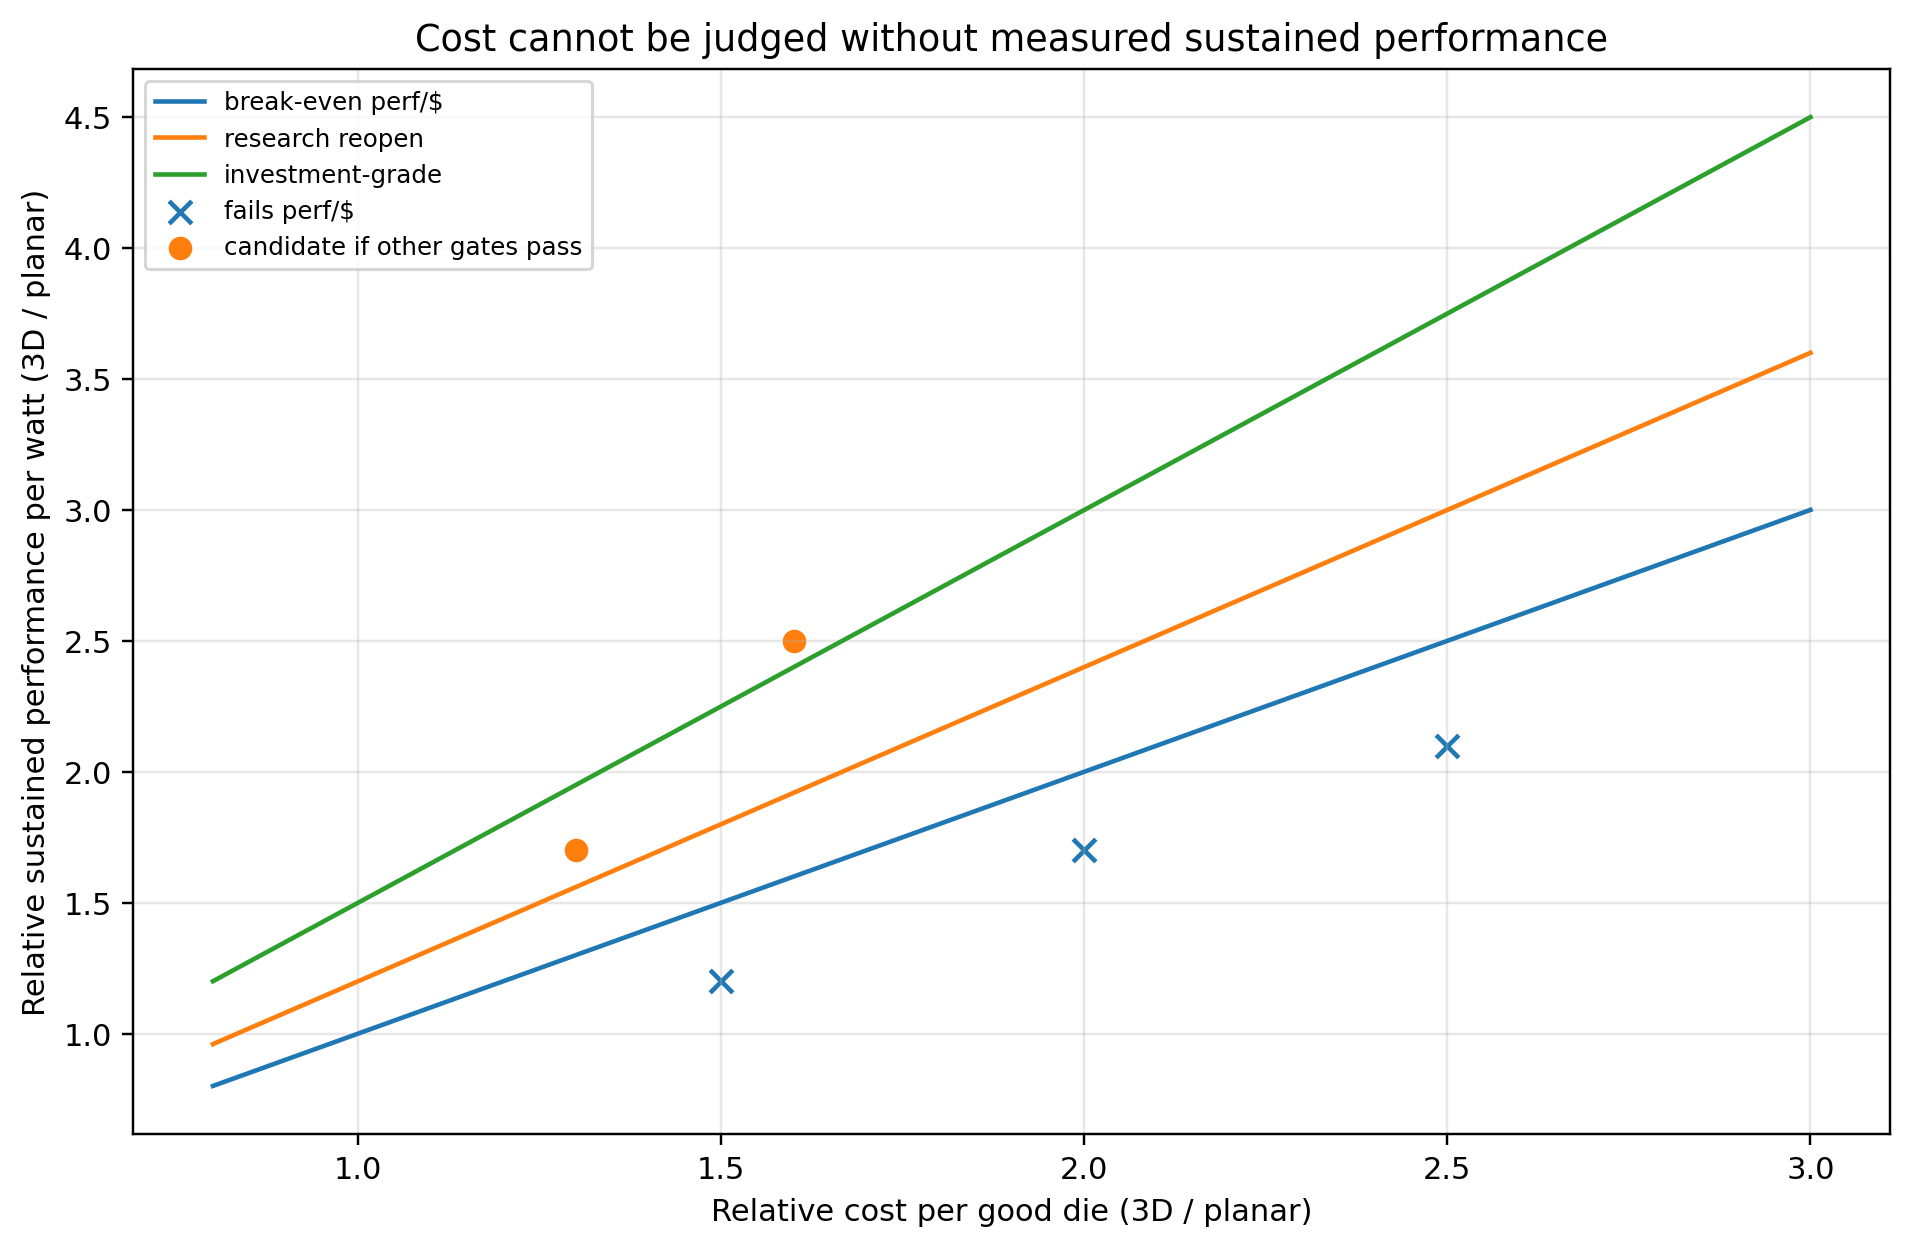
\includegraphics[width=0.78\linewidth]{fig_perf_cost.png}
\caption{The cost screen must be joint with sustained performance-per-watt. A fixed 1.5x cost multiplier is not a decision rule.}
\end{figure}

Suggested decision thresholds are not universal, but for screening:
\begin{longtable}{p{0.18\linewidth}p{0.24\linewidth}p{0.46\linewidth}}
\toprule
\textbf{Output} & \textbf{Condition} & \textbf{Interpretation}\\
\midrule
\endfirsthead
\toprule
\textbf{Output} & \textbf{Condition} & \textbf{Interpretation}\\
\midrule
\endhead
NO & $S_{value}<1$ & Worse value than baseline. Stop.\\
WATCH & $1\leq S_{value}<1.2$ & Interesting only if strategic constraints dominate. No investment thesis.\\
REOPEN & $1.2\leq S_{value}<1.5$ & Worth technical diligence if other gates pass.\\
ACTIONABLE & $S_{value}\geq1.5$ & Potentially actionable only with thermal, yield, EDA, and manufacturing proof.\\
\bottomrule
\end{longtable}

\section{Independent reproduction requires an open reference flow}
The portability gate cannot depend on two teams inside the same proprietary ecosystem. A minimum open reference flow should exist before anyone claims methodological portability.

\begin{figure}[H]
\centering
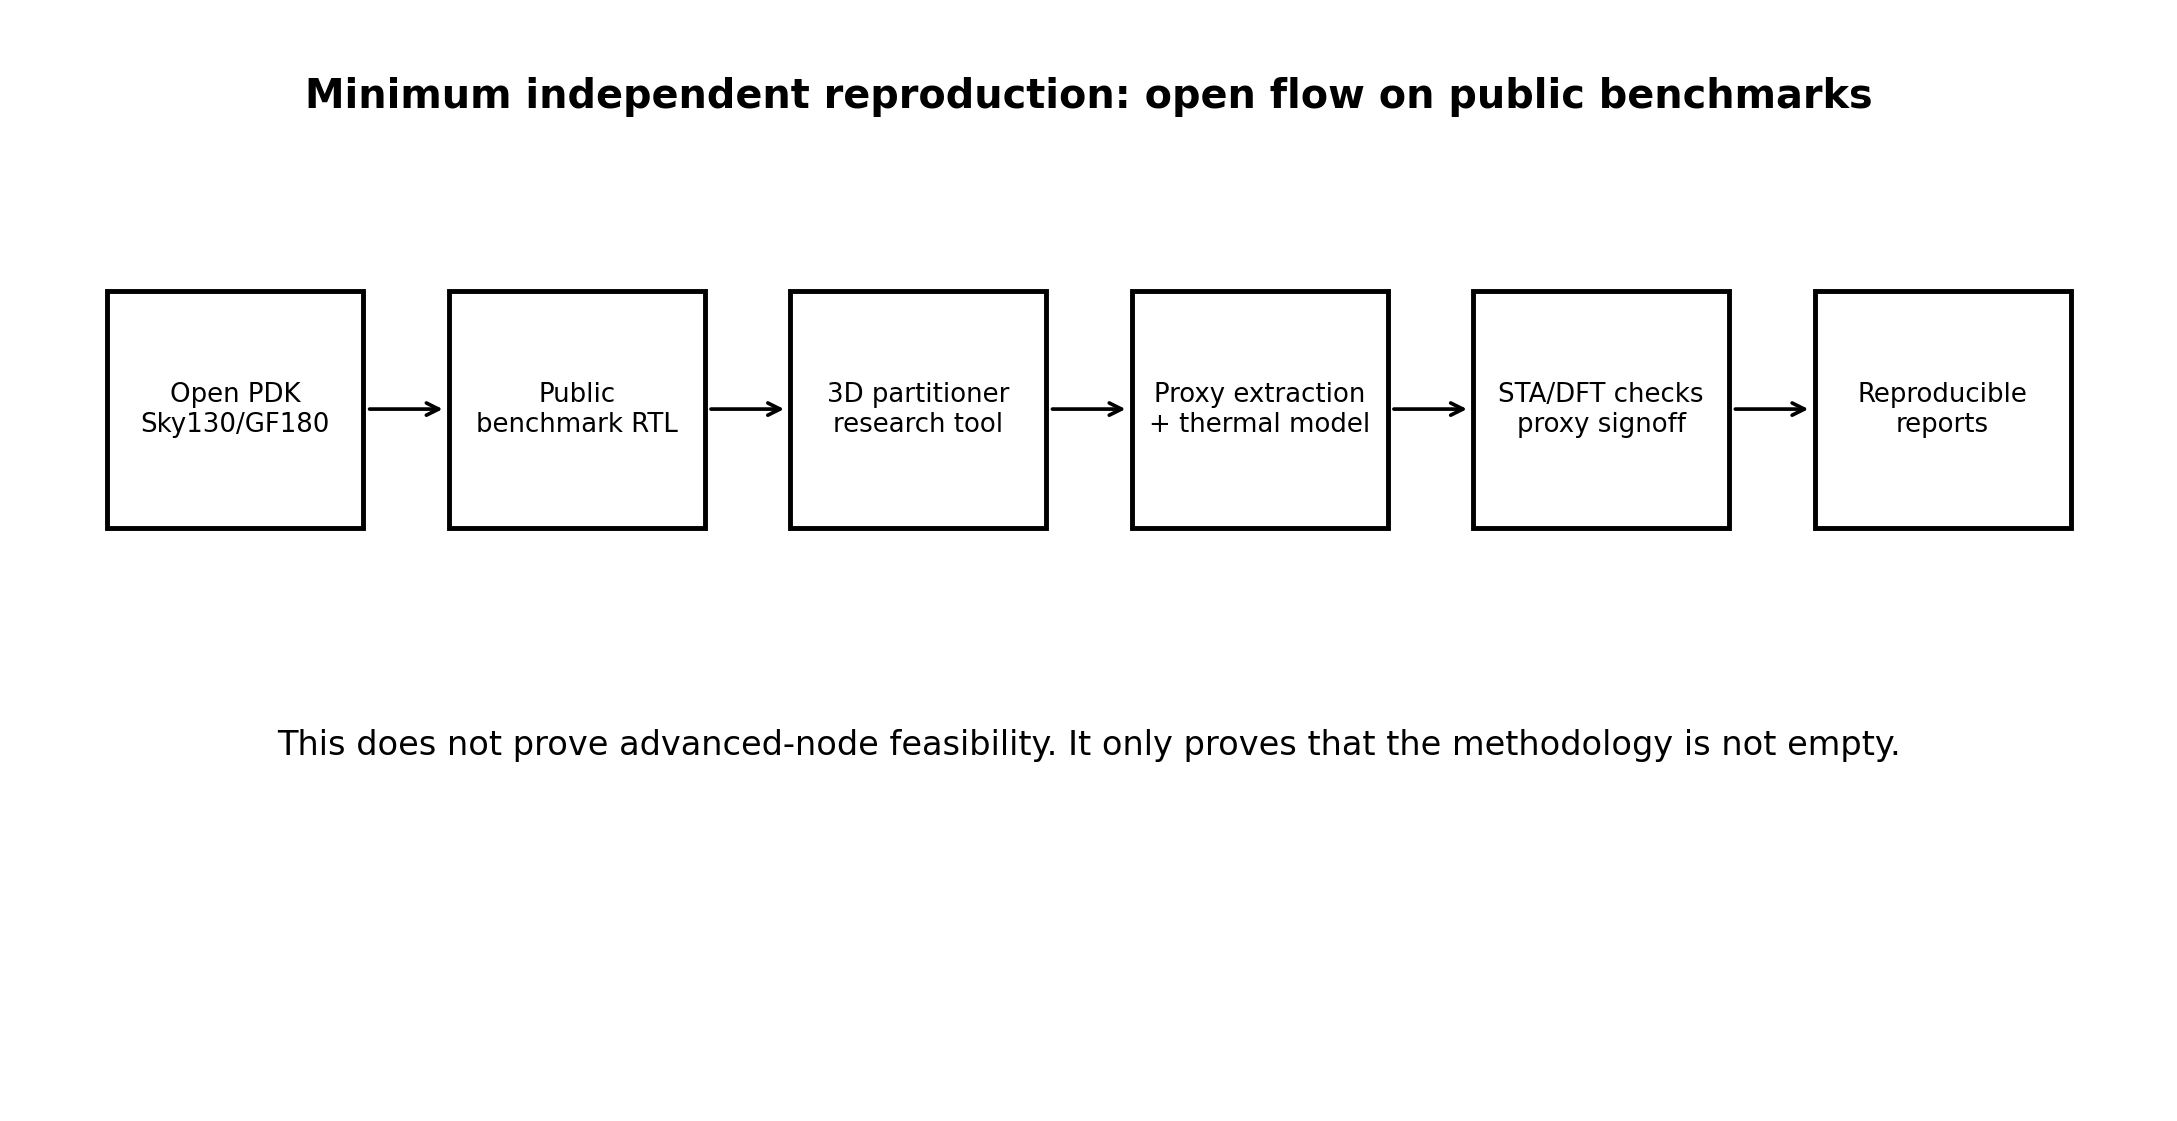
\includegraphics[width=0.98\linewidth]{fig_open_flow.png}
\caption{An open flow on mature public PDKs would not prove advanced-node viability, but it would prove that the methodology has executable content.}
\end{figure}

The reference flow should include:
\begin{itemize}
  \item permissive open-source license, reproducible container, and versioned inputs;
  \item public PDK demonstration, such as SkyWater 130 nm or GF180, with the caveat that these do not validate advanced-node parasitics;
  \item benchmark RTL/netlists and golden outputs;
  \item tier-aware partitioning prototype;
  \item proxy vertical parasitic and thermal models;
  \item checks for timing, DFT observability, and failure injection;
  \item public issue tracker and regression tests.
\end{itemize}

Such a flow would only answer ``is the methodology coherent?'' It would not answer ``does it work at 5 nm-class active logic?'' The latter still requires foundry data and silicon.

\section{Decision matrix}
A real decision screen must output YES, NO, WATCH, or REOPEN using observable metrics. Table \ref{tab:decision_matrix} gives the current screen.

\begin{longtable}{p{0.18\linewidth}p{0.28\linewidth}p{0.42\linewidth}}
\caption{Decision matrix for LogicFolding-style claims.}\label{tab:decision_matrix}\\
\toprule
\textbf{Evidence state} & \textbf{Decision} & \textbf{Reason}\\
\midrule
\endfirsthead
\toprule
\textbf{Evidence state} & \textbf{Decision} & \textbf{Reason}\\
\midrule
\endhead
Press release only & NO & Claims are not independent evidence.\\
Roadmap plus no silicon & NO & A roadmap can motivate research but not allocation.\\
Private demo, no data rights & NO/WATCH & Cannot distinguish real gain from hidden penalties.\\
Named foundry shuttle, no open data & WATCH & Gate 0 may be forming, but falsification remains weak.\\
Open reference flow only & RESEARCH ONLY & Methodology may be coherent; advanced-node feasibility unproven.\\
Shipping teardown with thermal and cost evidence & REOPEN & Product evidence can justify diligence.\\
Shipping teardown plus open/escrowed flow plus positive perf/\$ & ACTIONABLE DILIGENCE & Only here does an investment or engineering allocation become discussable.\\
\bottomrule
\end{longtable}

\section{Abandon and reopen rules}
\subsection{Abandon or ignore}
Ignore the hypothesis for trading and allocation if any of the following remains true:
\begin{enumerate}
  \item no shipping product has been torn down and measured;
  \item no foundry or integrated manufacturer is publicly or audibly tied to dual-active-logic stacking;
  \item no open or escrowed reference flow exists;
  \item no sustained workload thermal maps exist;
  \item vertical parasitic measurements do not satisfy path-level break-even;
  \item yield, DFT, test, and DPPM remain qualitative;
  \item the value score in Eq. \ref{eq:value} is not positive relative to platformized alternatives.
\end{enumerate}

\subsection{Reopen}
Reopen diligence only if at least one of the following occurs:
\begin{enumerate}
  \item a shipping phone or accelerator is independently shown to contain folded active logic and measured to sustain gains under thermal limits;
  \item a foundry announces or documents a dual-active-logic shuttle with data-access terms;
  \item an open reference flow demonstrates reproducible 3D partitioning, proxy thermal extraction, and verification on public benchmarks;
  \item teardown data reveals die size, package structure, thermal map, and cost model consistent with a positive $S_{value}$.
\end{enumerate}

\section{What remains academically useful}
Although the investment conclusion is negative, several research questions remain legitimate:
\begin{itemize}
  \item What topologies of critical paths have enough horizontal delay to justify vertical folding?
  \item Can public benchmark flows identify a restricted class of nets where folding is beneficial?
  \item What sensor/test structures would measure $K(r,r',t)$, $R_v$, $C_v$, $R_b$, and $C_b$ without exposing a full PDK?
  \item Can reduced-order APC be made useful for one or two observable quantities, rather than a full spatial field?
  \item What DFT architecture would make bonded active tiers diagnosable?
\end{itemize}

These are research questions, not product-plan milestones. Their output should be papers, open benchmarks, and test vehicles, not trading theses.

\section{Conclusion}
The third-pass red-team review forces the final downgrade. The document is no longer a portable methodology, no longer a falsification roadmap for ordinary researchers, and no longer a decision screen that implies near-term optionality. It is a no-action memo.

The default assumption should be that LogicFolding's claimed gains are either unproven or outweighed by hidden penalties. Backside power delivery, advanced packaging, chiplets, and foundry-platform roadmaps remain the lower-risk industrial path. LogicFolding should re-enter serious discussion only after public product evidence, auditable manufacturing access, or an open reference flow changes the information state.

\textbf{Final decision: Do not trade. Do not allocate. Do not treat as a viable alternative to backside power or conventional 3D packaging. Reopen only on shipping-teardown evidence or an auditable open/escrowed flow.}

\clearpage
\section*{Appendix A: Minimal public evidence packet}
\addcontentsline{toc}{section}{Appendix A: Minimal public evidence packet}
A credible public evidence packet should include:
\begin{longtable}{p{0.25\linewidth}p{0.62\linewidth}}
\toprule
\textbf{Category} & \textbf{Minimum contents}\\
\midrule
\endfirsthead
\toprule
\textbf{Category} & \textbf{Minimum contents}\\
\midrule
\endhead
Physical stack & Cross-section or credible package analysis showing folded active logic rather than ordinary packaging.\\
Path-time evidence & Ring oscillators, critical-path monitors, or timing measurements comparing folded and planar-equivalent paths.\\
Thermal evidence & Spatial thermal maps under sustained workloads with package and skin-temperature limits.\\
Parasitic evidence & Measured $R_v$, $C_v$, $R_b$, $C_b$, alignment, void, and defect distributions from test structures.\\
Yield/test evidence & Composite yield, post-bond failure analysis, DFT coverage, DPPM projection, and reliability cycling.\\
Cost evidence & Cost per good die with thinning, bonding, lithography, test, binning, and redundancy included.\\
Flow evidence & Reproducible partitioning, extraction, STA/thermal/DFT checks, and documented manual intervention.\\
\bottomrule
\end{longtable}

\section*{Appendix B: Operator notation is not enough}
\addcontentsline{toc}{section}{Appendix B: Operator notation is not enough}
A computational lithography or APC framework can be written abstractly as
\begin{equation}
\min_x \; \norm{\mathcal{F}_{\theta}(x)-y}^{2}+\lambda R(x),
\end{equation}
or
\begin{equation}
z_{k+1}=Az_k+Bu_k, \qquad y_k=Cz_k.
\end{equation}
These equations become operational only when $\mathcal{F}_{\theta}$, $R$, $A$, $B$, $C$, state dimension, measurement cadence, noise models, process drift, derivatives, constraints, and validation data are specified. Without those, the notation does not reduce engineering risk.

\section*{Appendix C: Stop-light summary}
\addcontentsline{toc}{section}{Appendix C: Stop-light summary}
\begin{longtable}{p{0.30\linewidth}p{0.16\linewidth}p{0.42\linewidth}}
\toprule
\textbf{Area} & \textbf{Status} & \textbf{Reason}\\
\midrule
\endfirsthead
\toprule
\textbf{Area} & \textbf{Status} & \textbf{Reason}\\
\midrule
\endhead
Public silicon evidence & Red & No independent shipping-product evidence in this memo.\\
Foundry access & Red & Gate 0 is an unavailable partnership, not a normal test.\\
Vertical parasitics & Red & Break-even requires measured data; fine-grained folding likely loses in many paths.\\
Thermal viability & Red & Needs workload-specific maps, not burst benchmarks or lumped estimates.\\
APC & Red & Spatial APC under sparse delayed metrology is unsolved.\\
EDA portability & Red & Requires open or escrowed reference flow; none is established here.\\
Cost/value & Red & Must be measured as sustained perf/W per cost per good die.\\
Research interest & Yellow & Worth academic work on restricted benchmarks and test vehicles.\\
Investment/action & Red & No trade, no allocation, no adoption.\\
\bottomrule
\end{longtable}

\clearpage
\begin{thebibliography}{99}
\bibitem{Huawei2026} Huawei. ``HUAWEI Presents the Tau ($\tau$) Scaling Law, Enabling Breakthroughs in Transistor Density and System Performance.'' May 25, 2026. \url{https://www.huawei.com/en/news/2026/5/ieee-iscas-tau-scaling}
\bibitem{Reuters2026} Che Pan, Eduardo Baptista, and Casey Hall. ``China's Huawei reveals chip design breakthrough amid US sanctions.'' Reuters, May 25, 2026. \url{https://www.reuters.com/world/asia-pacific/huawei-proposes-new-path-chip-development-amid-us-sanctions-2026-05-25/}
\bibitem{Intel18A} Intel Foundry. ``Intel 18A: See Our Biggest Process Innovation.'' Accessed May 27, 2026. \url{https://www.intel.com/content/www/us/en/foundry/process/18a.html}
\bibitem{TSMCA16} Taiwan Semiconductor Manufacturing Company. ``A16 Technology.'' Accessed May 27, 2026. \url{https://www.tsmc.com/english/dedicatedFoundry/technology/logic/l_A16}
\bibitem{SamsungSFF} Samsung Semiconductor. ``Samsung Showcases AI-Era Vision and Latest Foundry Technologies at SFF 2024.'' June 12, 2024. \url{https://semiconductor.samsung.com/news-events/news/samsung-showcases-ai-era-vision-and-latest-foundry-technologies-at-sff-2024/}
\bibitem{SamsungXCube} Samsung Semiconductor. ``Advanced Heterogeneous Integration.'' Accessed May 27, 2026. \url{https://semiconductor.samsung.com/foundry/advanced-package/advanced-heterogeneous-integration/}
\bibitem{Ai2015} Bing Ai, David Shan-Hill Wong, and Shi-Shang Jang. ``Stability analysis of semiconductor manufacturing process with EWMA run-to-run controllers.'' arXiv:1510.08946, 2015. \url{https://arxiv.org/abs/1510.08946}
\bibitem{UserRedTeam1} User-supplied red-team review. ``Portable 3D-Native LogicFolding Methodology.'' Uploaded May 27, 2026.
\bibitem{UserRedTeam2} User-supplied red-team review, second pass. ``Falsification Roadmap.'' Uploaded May 27, 2026.
\bibitem{UserRedTeam3} User-supplied red-team review, third pass. ``Decision Screen Roadmap.'' Uploaded May 27, 2026.
\end{thebibliography}

\end{document}
